\documentclass[a4paper,10pt]{article}
\usepackage[utf8]{inputenc}
\usepackage{graphicx}
\usepackage[sf, bf]{caption}

\setlength{\parindent}{1em}

\begin{document}
    \huge 
    \noindent
    \textbf{Brunn User Documentation}

    \normalsize

    \section{Bioclipse}
        The Bioclipse project is a Java-based, open source visual platform for
        chemo- and bioinformatics built upon the Eclipse Rich Client Platform
        (RCP). Brunn is a plugin for Bioclipse.

        \subsection{Editors and Views}
            Bioclipse is made up of editors and views. Editors are for editing
            things. Items can be opened in an editor, changed and then saved and
            the editor closed. A view can listen to, and change appearence
            according to, the current selection. For example the Properties view
            shows the properties of the item currently selected. Figure
            \ref{editorsAndViews} shows an example of what are views and what
            are editors in a standard Brunn window.
            
            \begin{figure}[htbp]
                \begin{center}
                    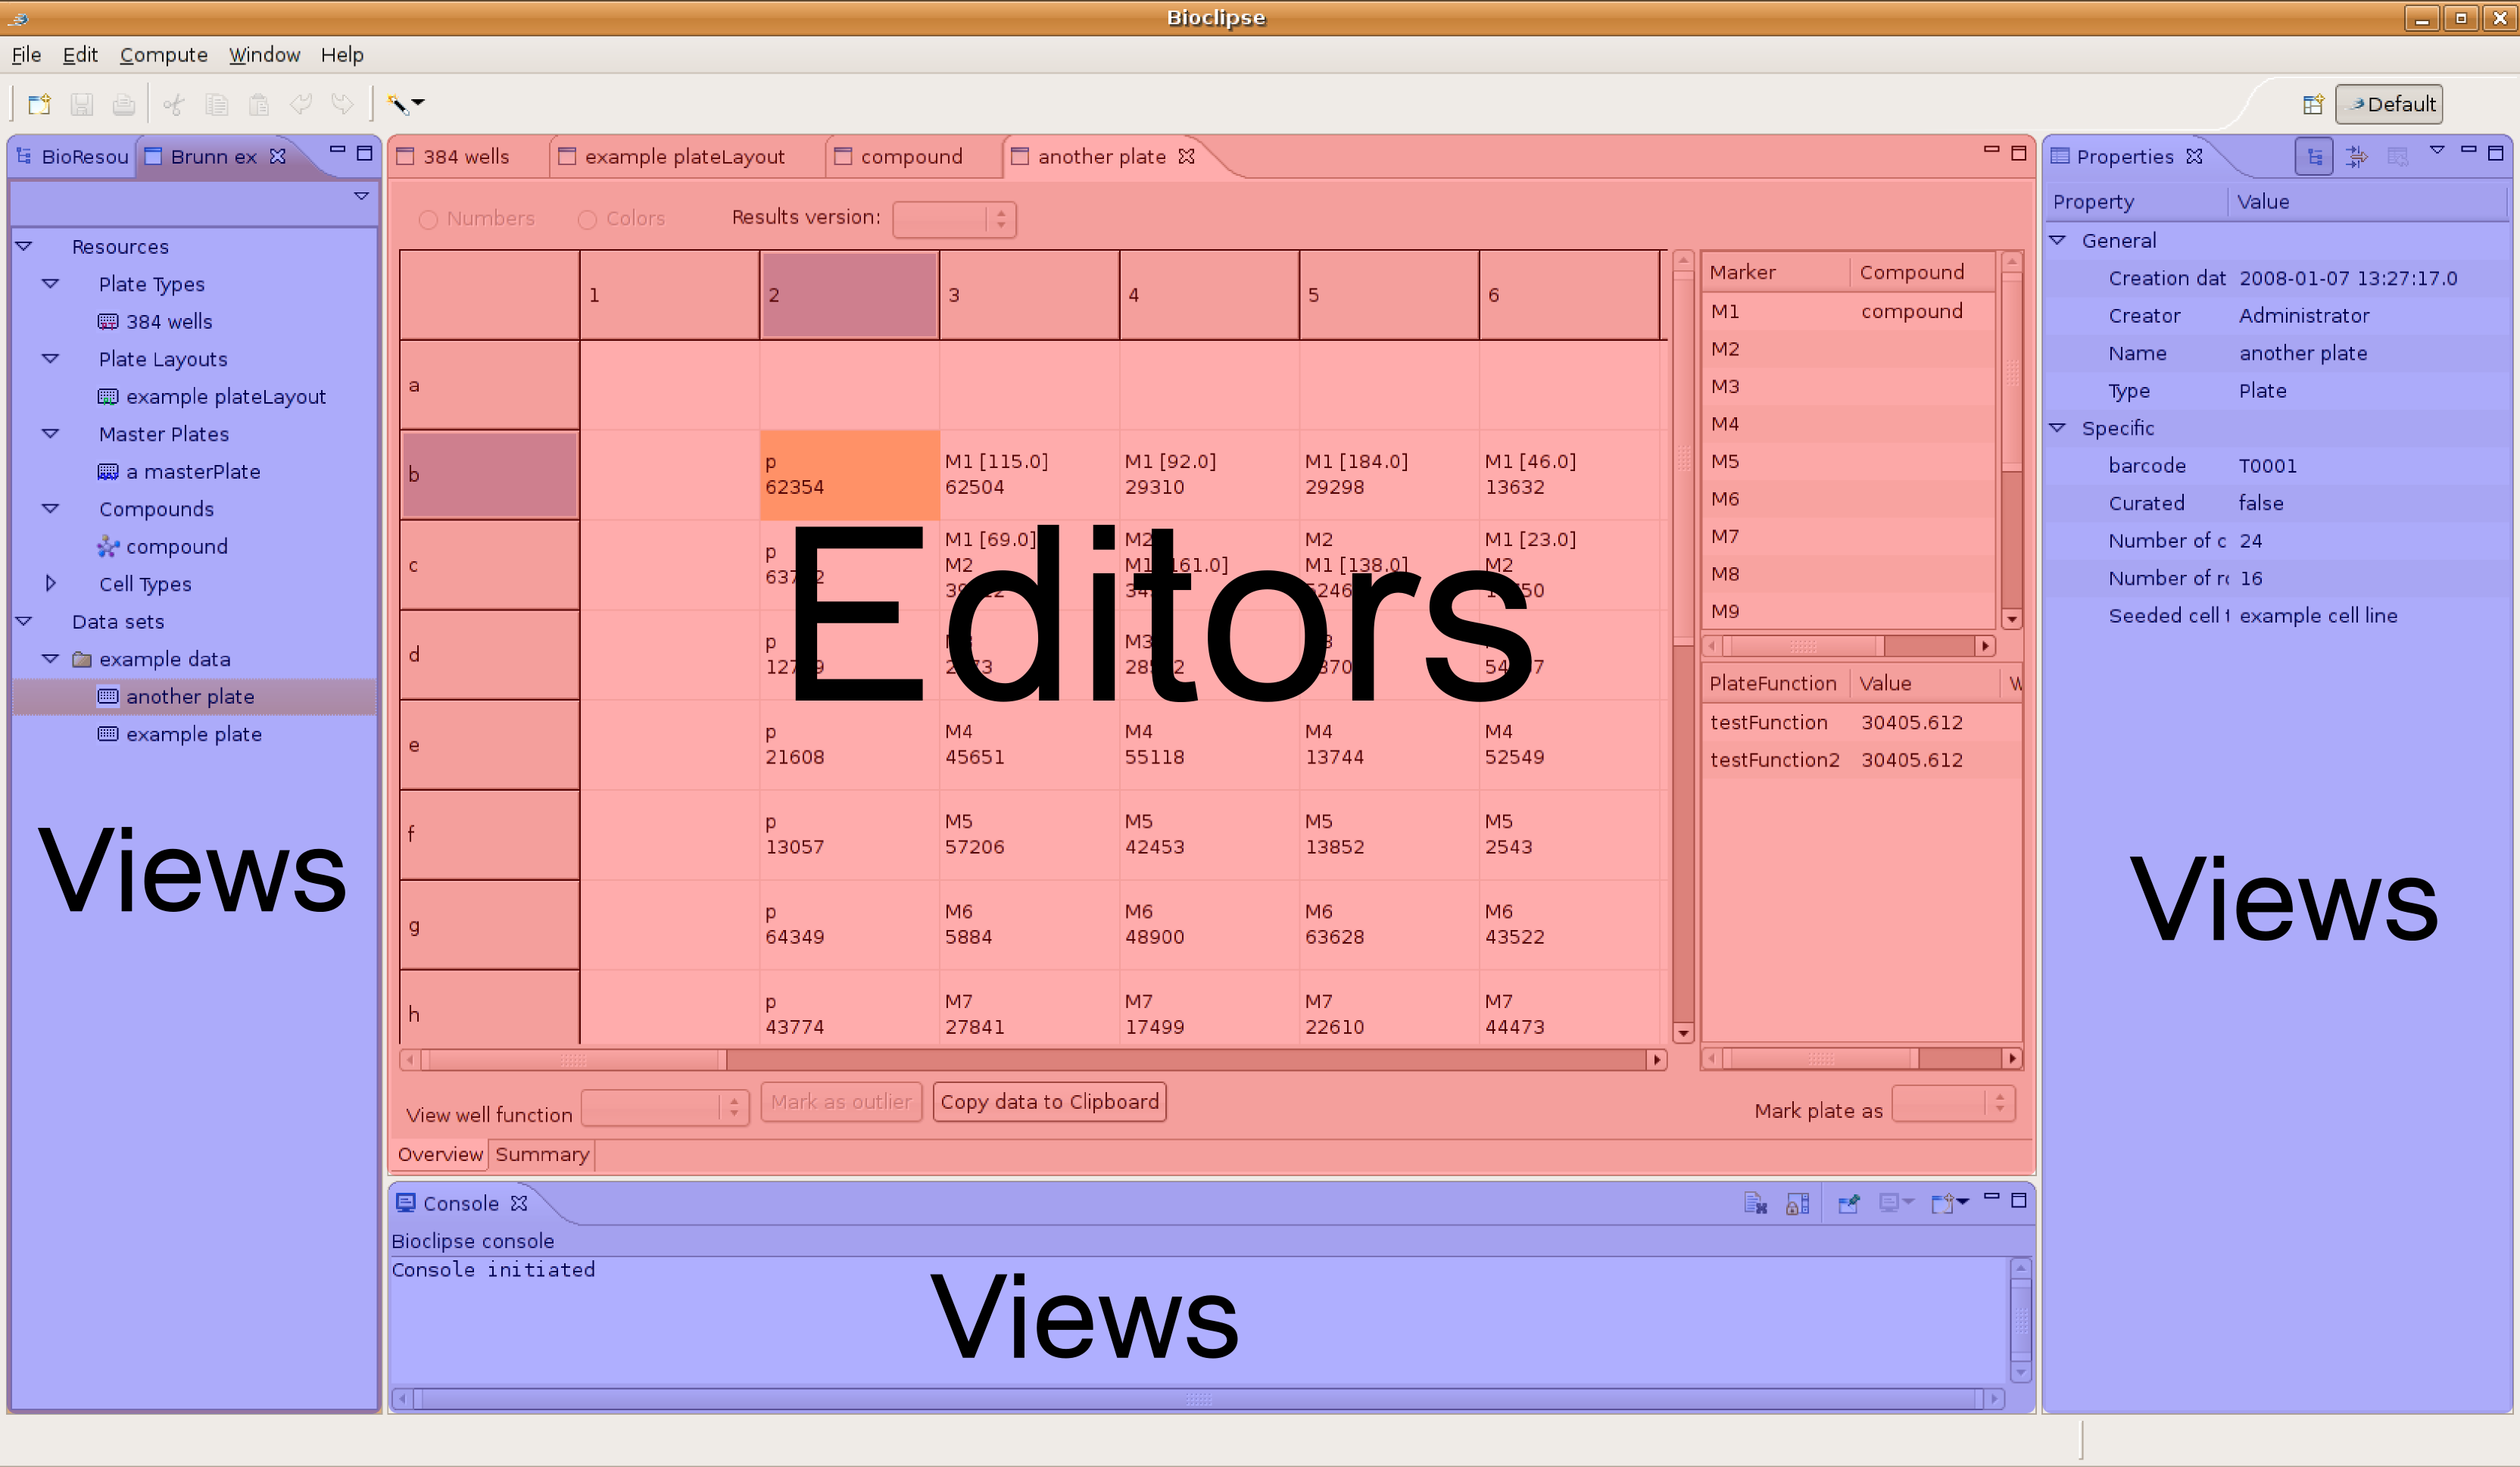
\includegraphics[width=1\textwidth]{images/EditorsViews.png}
                \end{center}
                \caption{\textit{The Bioclipse workspace consists of editors
                                 and views. The editors are piled in the
                                 middle and the views can be moved around.}}
                \label{editorsAndViews}
            \end{figure}

        \subsection{Two ``hidden'' but important menus}

            There are two sorts of menus in Bioclipse that can be
            hard to find. Figure \ref{viewMenu} indicates them. One contains
            operations coupled to a view and can be found (in a view that has
            such a menu) when clicking a little triangle in the upper right
            corner of the view. The other switches between different tabs in a
            multipage editor. Not all editors have multiple pages.
            \begin{figure}[htbp]
                \begin{center}
                    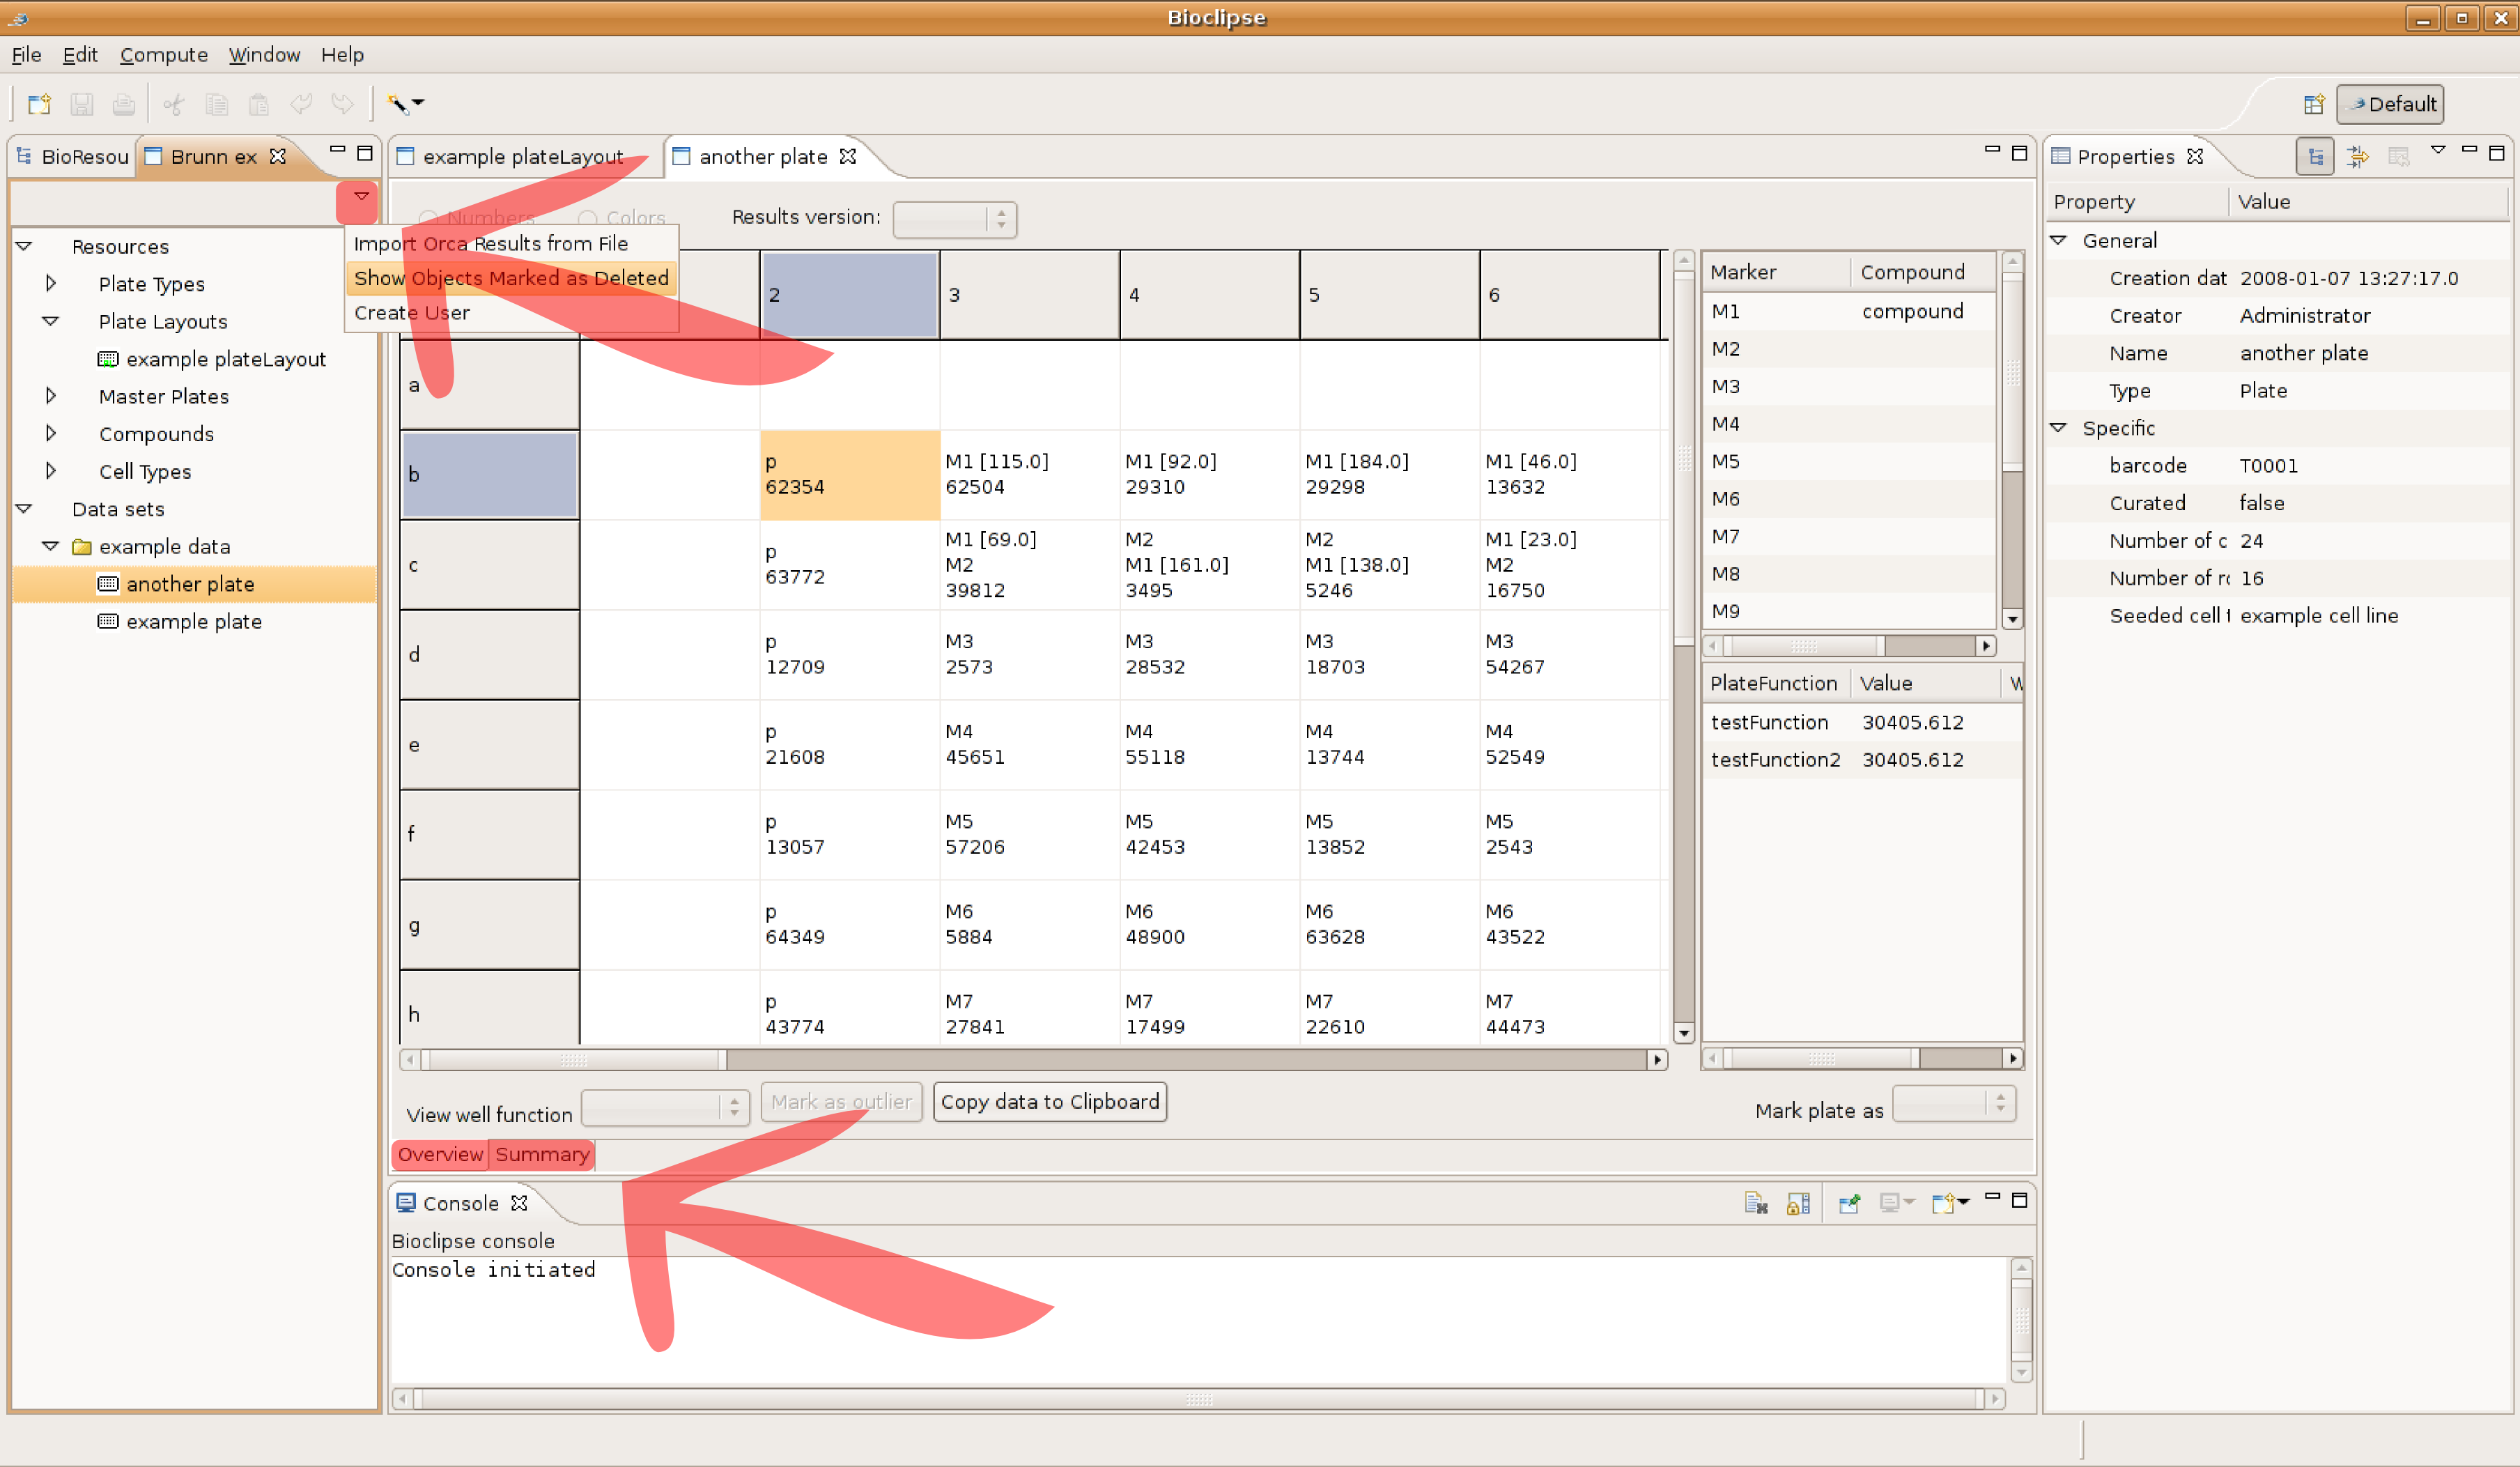
\includegraphics[width=1\textwidth]{images/twoMenues.png}
                \end{center}
                \caption{\textit{A view can have a menu. They are very
                    convenient but can be hard to spot the first time. They are
                    just little triangles in the corner of the view. Editors
                    can have multiple pages but this feature can also be hard
                    to spot. The tabs at the bottom of the editor switch
                    between pages.}}
                \label{viewMenu}
            \end{figure}

    \section{Brunn}
        
         \begin{minipage}{1\textwidth}
            A few general tips for the Brunn user:
            \begin{itemize}
                \item Double-clicking an item opens it up for editing
                \item Right-clicking often opens up a context menu with
                    operations. If you wonder about how to do somehing, try
                    right clicking.
            \end{itemize}
         \end{minipage}

         \subsection{Installation and Set-Up}
         \texttt{TODO:}Write stuff here

         \subsection{The Brunn Explorer View} 
            \begin{figure}
                \begin{center}
                    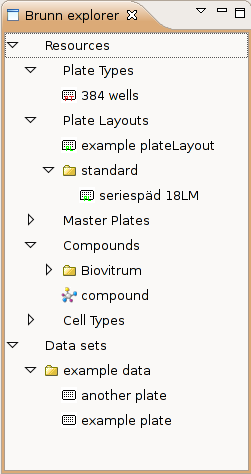
\includegraphics[width=.2\textwidth]
                                    {images/explorerView.png}
                \end{center}
                \caption{\textit{The Brunn Explorer view is used to browse the
                    system. The contents are sorted in fixed super folders for
                    each type and can be further sorted into moveable sub
                    folders } \texttt{TODO: Switch to new image with new icons
                    and with the context menu showing}}
                \label{explorerView}
            \end{figure}

            \noindent
            The first time Brunn is started the Brunn Explorer View (Figure
            \ref{explorerView}) might not be visible. It can be made visible by
            clicking: \texttt{Window$\rightarrow$Show
            View$\rightarrow$Other\ldots} and under Brunn, choose Brunn
            Explorer. 

            Double-clicking something in the Explorer View opens that item in
            an editor. New items are created from the Explorer View. The
            various items of the tree have context menus that appear when
            right-clicking. For example, folders can be created and items can be
            dragged and dropped into and out of them. Figure \ref{labWork}
            explains how the different items in the tree fit in to what is done
            in the lab.  

            Almost nothing can be deleted in Brunn. However, things can be
            marked as deleted, meaning that they won't show up unless the menu
            alternative \texttt{Show Objects Marked as Deleted} is choosen in
            the Brunn Explorer views menu. In this menu, there is also a wizard
            for importing result data and a way to create a new user account.
            The alternatives to show objects marked as deleted and to create
            users are only there if the logged-in user has administrator
            level access.
        
        \begin{figure}[htbp]
            \begin{center}
                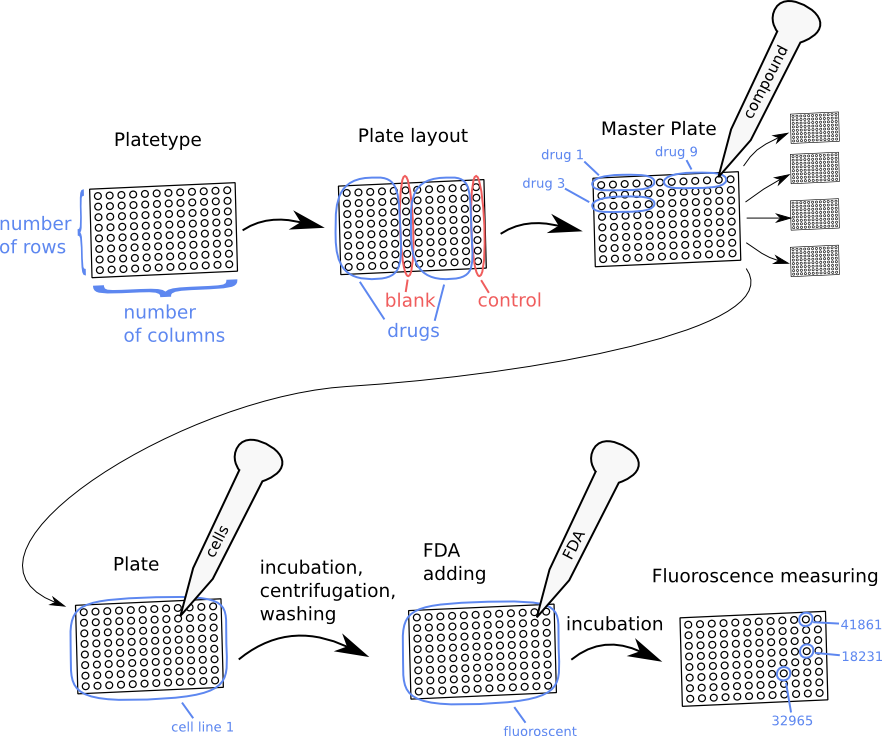
\includegraphics[width=1\textwidth]{images/labWork.png}
            \end{center}
            \caption{\textit{A description of how the items of Brunn fit into
                             the work performed in the lab. In the system, a
                             plate type defines the size, number of columns and
                             rows of a plate. A plate layout defines where on
                             the plate the controls and the compounds are to be
                             placed. Based upon this plate layout, a number of
                             equal plates are made, conforming to a so-called
                             “master plate” that defines which drugs are placed
                             in which wells. Each one of this plates corresponds
                             to a real life plate with an unique barcode
                             number. }}
            \label{labWork}
        \end{figure}

        \subsection{Creating items}
            New items are created by right-clicking a folder that is either the
            top folder for the sort of item to be created or one of it's
            subfolders, and then choosing a create operation. This opens a
            dialog where things special for that sort of item can be entered. 

            In order to create a plate layout, start by right-clicking the
            \texttt{Plate Layouts} folder and choose \texttt{Create Plate
            Layout}. In the dialog that shows up, choose one plate type to base
            the plate layout on, and enter a name for your new plate layout.
            Then click \texttt{Ok} to create the plate layout.

        \subsection{Plate Type} A plate type defines the size of a plate. It
            simply holds the number of rows and columns of a plate. 

        \subsection{Plate Layout}
            A plate layout defines which wells on a plate should be used for
            compounds, which should be used for controls, and which should just
            be left empty. The plate layout is also where calculation functions
            are defined. For example, survival index or variation over the
            wells marked as positive control are specified in the plate layout.

            \begin{figure}[htbp]
                \begin{center}
                    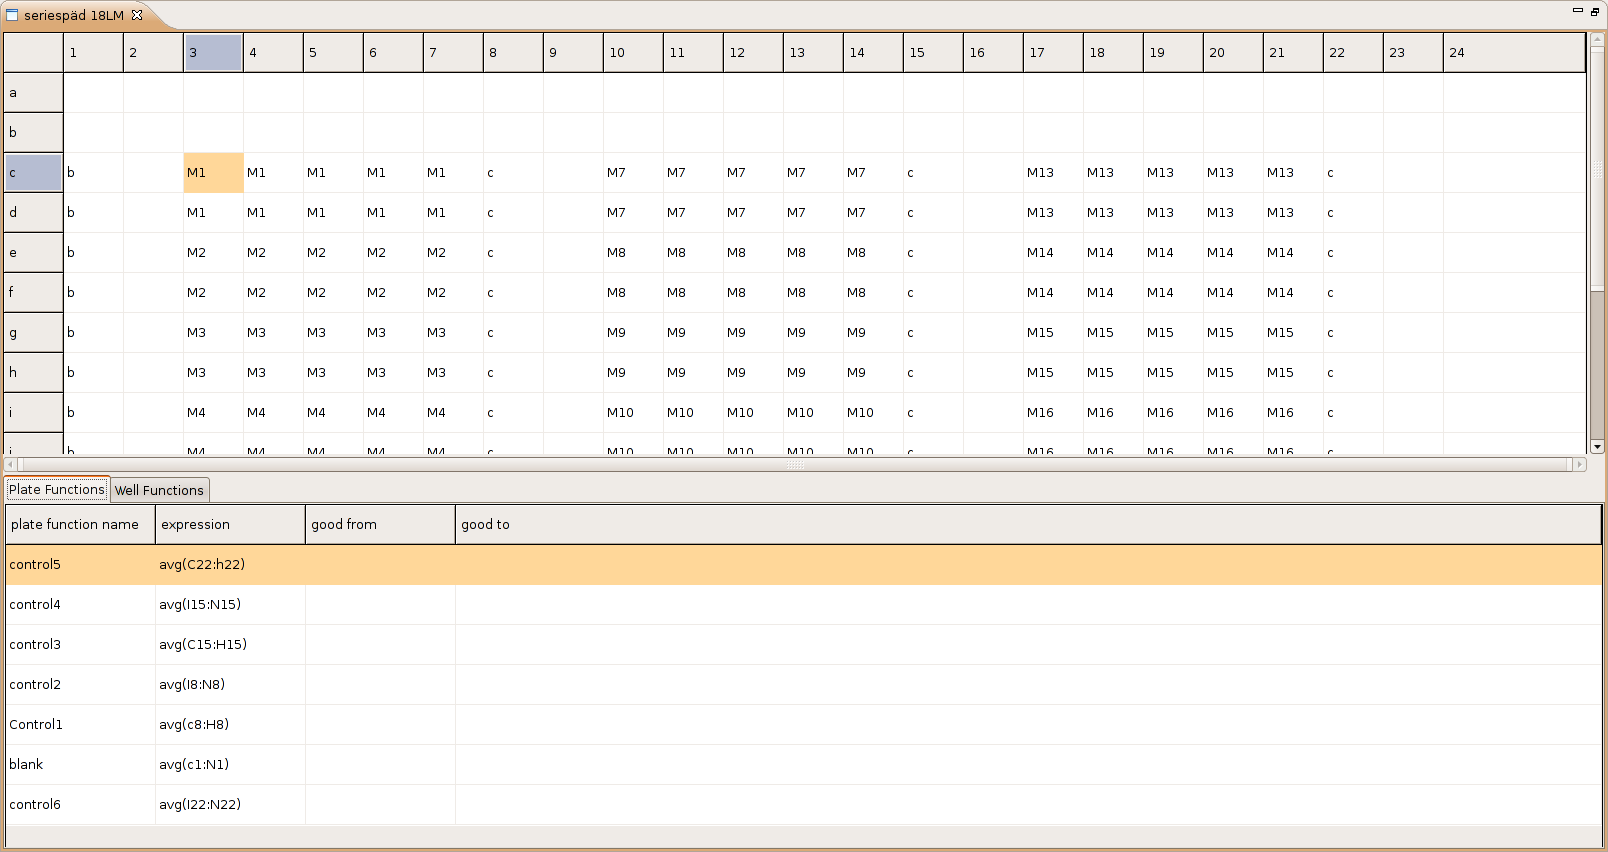
\includegraphics[width=1\textwidth]
                                    {images/plateLayoutEditor.png}
                \end{center}
                \caption{\textit{The platelayouteditor}}
                \label{platelayoutEditor}
            \end{figure}

            \subsubsection{Adding markers to a plate layout}
                Markers are used for labeling wells for different use. Brunn
                has 5 types of markers (see table \ref{markersTable}).

                \begin{table}
                    \begin{center}
                        \begin{tabular}{l|l}
                            Marker & Description \\
                            \hline
                            b & Blank.           \\
                            c & Control.         \\
                            p & Positive control \\
                            s & Solvent          \\
                            M1 \ldots M\textit{n} & Substance marker. \\ 
                                                  & Each number corresponds to
                                                    one substance. \\
                        \end{tabular}
                    \end{center}
                    \caption{\textit{The different well markers used in Brunn}}
                    \label{markersTable}
                \end{table}
                
                Labeling a well with a marker is done by right-clicking the
                well in the plate layout editor and choosing the marker to
                label with. Multiple wells can be labeled at once by first
                selecting a number of wells and then right-clicking and
                choosing a marker. De-labeling is similar. When right-clicking a
                well with a marker an option to remove marker will appear in the
                right-click menu.

            \subsubsection{Defining calculation functions on a plate layout}
                The plate layout editor is also the place to define
                calculations. For example the expression for survival index
                (SI):
                \begin{equation} SI = ? \mbox{ \texttt{TODO: write expression} }
                \label{si} \end{equation}
                is added here. Brunn works with two groups of functions for
                calculations. Plate functions are coupled to a plate and should
                be used for things like average values of controls or
                variations for blanks. Well functions are coupled to a well and
                should be used for things like SI (equation \ref{si}).
                
                The bottom part of the editor consists of a listing of added
                functions. To add a new one, simply right-click and choose
                \texttt{add function}. There are a few mathematical functions
                (Table \ref{functions}) defined that can be used. 

                \begin{table}
                    \begin{center}
                        \begin{tabular}{l|l}
                            Function & Description \\
                            \hline
                            \texttt{sum} &    Sum of the given values \\
                            \texttt{avg} &    The average of the
                                              given values \\
                            \texttt{stddev} & The standard deviation 
                                              of the given values \\
                        \end{tabular}
                    \end{center}
                    \caption{\textit{Listing of predefined functions that can
                                     be used for calculations}}
                    \label{functions}
                \end{table}
                
                Well functions can be added by first switching to the well
                functions tab and then selecting a couple of wells that should
                be given well functions and then clicking \texttt{add function}
                just as with the plate functions. Here a little trick can be
                used: The variable \texttt{well} will be translated to the name
                of the current well. 

                \texttt{TODO: Add example using SI as example}
        \subsection{Master Plate}
            A master plate defines which compound marker correspond to which
            compound and with what concentration.
            
            \subsubsection{Defining compound for a compound marker}
                The masterplate editor is used for connecting substance markers
                with substances. It has functionality for creating dilution
                series. Conecting a substance to a marker is done by dragging
                the substance from the Brunn Explorer and into the list of
                markers at the bottom part of the editor. A dialog will 
                ask for information of how to perform dilution.

                \texttt{TODO: add illustration of dialog}
        \subsection{Plate}
            A plate corresponds to a real world plate. This connection is made
            by a barcode. So when creating a plate an unique barcode for the new
            plate needs to be given. 

            \subsubsection{The plate editor}
                After results has been imported for a plate (see
                \ref{importingResult}) the plate editor can be used for
                inspecting it. The plate editor has three tabs. Each of
                them contains a button for copying the table shown in that tab
                to clipboard.

                \paragraph{The overview tab}
                    The overview tab shows the result values for the plate in
                    the same order as the actual plate. Each well has a few
                    rows. The first row is the data value. After that come
                    substance markers and concentrations. At the bottom of the
                    editor is a row of buttons. The first is a combo box where
                    the well function being shown for the wells can be
                    changed. Then there is a button for marking a well as
                    outlier. When a well is marked as outlier it will not be
                    used in any calculations. In the right part of the editor
                    is a list of substance markers and which compound it
                    corresponds to, and below are all the plate functions
                    listed.

                \paragraph{The summary tab}
                    The summary tab contains a table listing, for each well
                    with compounds, the compounds names, concentrations, all
                    well functions values and a CV\% for the replicates. This
                    tab also has a button for marking a well as an outlier. 

                \paragraph{The average tab}
                    The average tab looks very much like the summary tab but
                    instead of showing values for each well, it shows the average
                    for each group of replicates. Since each row in this table
                    corresponds to an average for many wells, there is no button
                    for marking a well as outlier here.

        \subsection{Importing result data}
        \label{importingResult}
            Importing results is done in a dialog which can be found in the
            Brunn Explorer view's menu. Recall that figure \ref{viewMenu} at
            page \pageref{viewMenu} shows where this menu can be found. The
            dialog is designed to accept files of three different formats.  
            
            \texttt{TODO: Describe or add examples of the three file formats}
\end{document}

